\chapter{Forward and Inverse Kinematics}\label{chap:kinematics}
In order to plan a robot's movements, we have to understand the relationship between the actuators that we can control and the robot's resulting position in the environment. For static arms, this is rather straightforward: if we know the position/angle of each joint, we can calculate the position of its end-effectors using trigonometry. This process is known as \emph{forward kinematics}. \index{Forward Kinematics} If we want to calculate the position each joint needs to be at, we need to invert this relationship. This is known as inverse kinematics. \index{Inverse Kinematics} For mobile robots, this process is usually more involved, as speeds need to be integrated, which we refer to as \emph{odometry}\index{Odometry}.

The goals of this chapter are:

\begin{itemize}
\item introduce coordinate systems and their transformations,
\item to introduce the forward kinematics of simple arms and mobile robots
\item understand the concept of holonomy,
\item show how solutions for the inverse kinematics for both static and mobile robots can be derived,
\item provide an intuition on the relationship between inverse kinematics and path-planning.
\end{itemize}

\section{Coordinate Systems and Frames of Reference}\label{sec:coordsystems}
\screencast{http://youtu.be/klBJi-MEeNQ}{coordinatesystem}
Every robot assumes a position in the real world that can be described by its position (x, y and z) and orientation (pitch, yaw and roll) along the three major axes of a Cartesian Coordinate system (See also Section~\ref{sec:dof}, ``Degrees of freedom''). Such a coordinate system is shown in Figure~\ref{fig:coordinatesystem}. Note that the directions and orientations of the coordinate axes are arbitrary. This books uses the ``right hand rules'', which are illustrated in Figure~\ref{fig:coordinatesystem} to determine axes labels and directions throughout. Pitch, yaw, and roll, are also known as bank, attitude, and heading in other communities. \index{Pitch}\index{Yaw}\index{Roll}\index{Bank}\index{Attitude}\index{Heading} This makes sense, considering the colloquial use of the word ``heading'', which corresponds to a rotation around the z-axis of a vehicle driving on the x-y-plane.

\begin{figure}
	\centering
		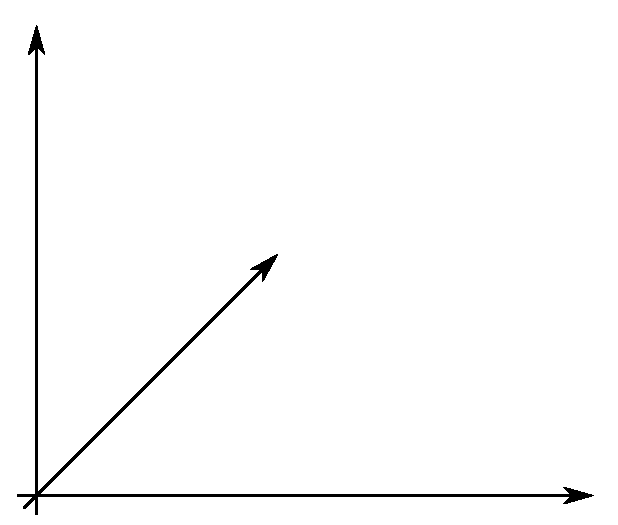
\includegraphics[width=0.8\textwidth]{figs/coordinatesystem}
	\caption{A coordinate system indicating the direction of the coordinate axes and rotation around them. These directions have been derived using the right-hand rules.}
	\label{fig:coordinatesystem}
\end{figure}

Defining all three position axes and orientations might be cumbersome. What level of detail we care about, where the origin of this coordinate system is, and even what kind of coordinate system we chose, depends on the specific application. For example, a simple mobile robot would typically require a representation with respect to a room, a building, or the earth's coordinate system (given by the longitude and latitude of each point on the earth), whereas a static manipulator usually has the origin of its coordinate system at it's base. More complicated systems, such as mobile manipulators or multi-legged robots, make life much easier by defining multiple coordinate systems, e.g.\ one for each leg and one that describes the position of the robot in the world frame. These local coordinate systems are known as \emph{Frames of Reference}\index{Frame of Reference}.
An example of two nested coordinate systems is shown in Figure~\ref{fig:nestedcoords}. In this example, a robot located at the origin of $x',y'$ and $z'$ might plan its motions in its own reference frame, which can then be expressed in the coordinate system $x$, $y$ and $z$ by performing a translation and a rotation as we will later see.

Depending on it's degrees-of-freedom, that is the number of independent translations and rotations a robot can achieve in Cartesian space, it is also customary to ignore components of position and orientation that remain constant. For example a simple floor-cleaning robot's pose might be completely defined by it's $x$ and $y$ coordinates in a room as well as its orientation, i.e.\ its rotation around the $z$-axis.


\begin{figure}
	\centering
		
\includegraphics[width=\textwidth]{figs/frameofreference.png}
	\caption{Two nested coordinate systems (frames of reference).}
	\label{fig:nestedcoords}
\end{figure}

\subsection{Matrix notation}
Given some kind of fixed coordinate system, we can describe the \emph{position} of a robot's end-effector by a $3x1$ position vector. As there can be many coordinate systems defined on a robot and the environment, we identify the coordinate system a point relates to by a preceeding super-script, e.g., $ ^AP$ to indicate that point $P$ is in coordinate system $\{A\}$. Each point consists of three elements $ ^AP=[p_x p_y p_z]^T$.

More formally, $^AP$ is a linear combination of the three basis vectors that span $A$:
\begin{equation}
^AP=p_x\left(\begin{array}{c}1\\0\\0\end{array}\right)+p_y\left(\begin{array}{c}0\\1\\0\end{array}\right)+p_z\left(\begin{array}{c}0\\0\\1\end{array}\right)\label{eq:basis}
\end{equation}

\screencast{http://youtu.be/QdHO_9M8-UI}{frameofreference}
As we know, not only the position of the robot is important, but also its orientation. In order to describe the orientation of a point, we will attach a coordinate system to it. Let $ \hat{X}_B, \hat{Y}_B$ and $ \hat{Z}_B$ be unit vectors that correspond to the principal axes of a coordinate system $\{B\}$. When expressed in coordinate system $\{A\}$, they are denoted $^A\hat{X}_B, ^A\hat{Y}_B$ and $ ^A\hat{Z}_B$. In order to express a vector that is given in one coordinate system in another, we need to project each of its components to the unit vectors that span the target coordinate system. For example considering only the axis $^A\hat{X}_B$

\begin{equation}\label{eq:projection}
^A\hat{X}_B=(\hat{X}_B\cdot\hat{X}_A, \hat{X}_B\cdot\hat{Y}_A,\hat{X}_B\cdot\hat{Z}_A)^T
\end{equation}
consists of the projections of $\hat{X}_B$ onto $\hat{X}_A$, $\hat{Y}_A$ and $\hat{Z}_A$. Here,  $|\cdot|$ denotes the scalar product (also known as dot or inner product).  Note that all vectors in (\ref{eq:projection}) are unit vectors, i.e.\ their length is one. By definition of the scalar product, $A\cdot B=\|A\|\|B\|\cos \alpha=\cos \alpha$, indeed reduces the projection of $\hat{X}_B$ onto the unit vectors of $\{A\}$. This projection is illustrated in Figure~\ref{fig:projection}.

\begin{figure}
	\centering
		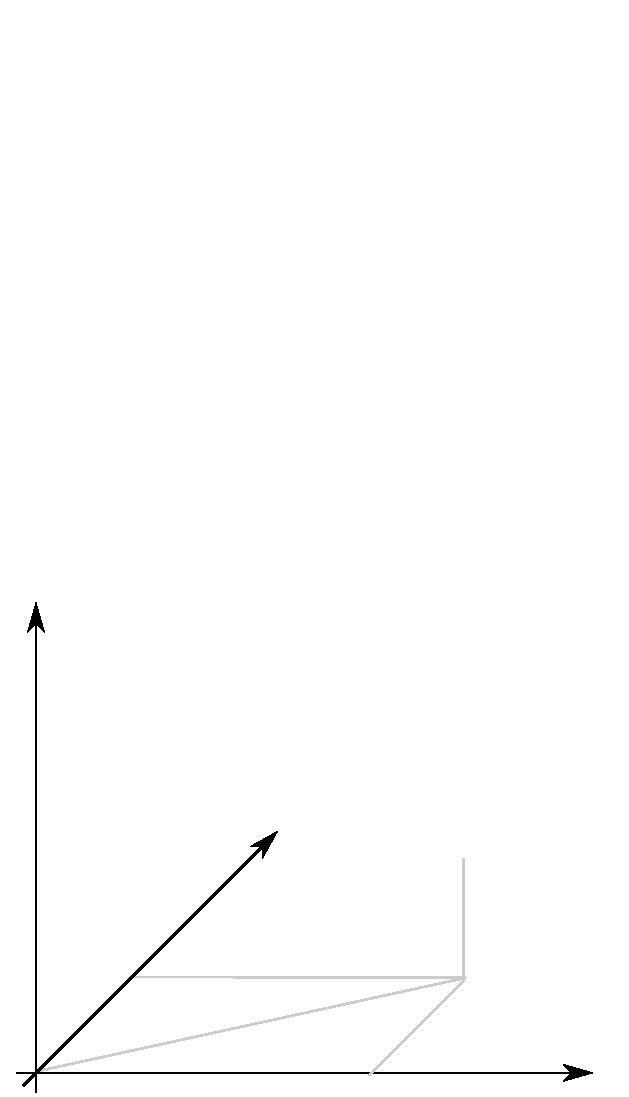
\includegraphics[width=0.8\textwidth]{figs/projection.png}
	\caption{Top: A coordinate system $\{B\}$ with position given by $^AP$ and orientation given by $\hat{X}_B$, $\hat{Y}_B$, and $\hat{Z}_B$. Bottom:
	The projection of the unit vector $\hat{X}_B$ onto the unit vectors that span coordinate system $\{A\}$ after moving $\{B\}$ into the origin of $\{A\}$. As all vectors are unit vectors, $A\cdot B=\|A\|\|B\|\cos \alpha=\cos \alpha$. }
	\label{fig:projection}
\end{figure}

We can now do this for all three vectors that span coordinate system $\{B\}$ and stack these three vectors together into a 3x3 matrix to obtain the rotation matrix
%
\begin{equation}
^A_BR=[^A\hat{X}_B \quad ^A\hat{Y}_B \quad ^A\hat{Z}_B]
\end{equation}
%
which describes $\{B\}$ relative to $\{A\}$. It is important to note that all columns in $ ^A_BR$ are unit vectors, so that the rotation matrix is orthonormal. This is important as this allows us to easily obtain the inverse of $ ^A_BR$ as $ ^A_BR^T$ or
$ ^B_AR=^A_BR^T$.

Why the unit vectors of a coordinate system $\{B\}$ expressed in coordinate system $\{A\}$ actually make up a rotation matrix, can be easily seen when re-arranging equation~\ref{eq:basis} in matrix form
\begin{equation}
^AP=\left(\begin{array}{ccc}1 & 0 & 0\\0 & 1 & 0\\0 & 0 & 1\end{array}\right)\left(\begin{array}{c}p_x\\p_y\\p_z\end{array}\right),
\end{equation}
where the rotation matrix is nothing but the identity as both points already are in the same coordinate system.

We have now established how to express the orientation of a coordinate system using a rotation matrix. Usually, coordinate systems don't lie on top of each other, but are also displaced from each other.
Together, position and orientation is known as a \emph{frame},\index{Frame} which is a set of four vectors, one for the position and three for the orientation, and we can write
%
\begin{equation}
\{B\}=\{^A_BR, ^AP\}
\end{equation}
%
to describe the coordinate frame $\{B\}$ with respect to $\{A\}$ using a vector $^AP$ and a rotation matrix $^A_BR$. Robots usually have many such frames defined along their bodies.

\subsection{Mapping from one frame to another}
\screencast{http://youtu.be/NsiJNvsuO3s}{rotationmatrix}
Having introduced the concept of frames, we need the ability to map coordinates in one frame to coordinates in another frame. For example, lets consider frame $\{B\}$ having the same orientation as frame $\{A\}$ and sitting at location $^AP$ in space. As the orientation of both frames is the same, we can express a point $ ^BQ$ in frame $\{A\}$ as
%
\begin{equation}
^AQ=^BQ+^AP
\end{equation}
%
Actually, adding two vectors that are in different reference frames, i.e., $ ^BQ+^AP$, is only possible if both of them have the same orientation. We can, however, convert from one reference frame to the other using the rotation matrix:

\begin{equation}
^AP=^A_BR^BP
\end{equation}
%
and therefore solve the mapping problem regardless of the orientation of $\{A\}$ to $\{B\}$:
\begin{equation}
^AQ=^A_BR^BQ+^AP
\end{equation}
Using this notation, we can see that leading subscripts cancel the leading superscripts of the following vector/rotation matrix. Whereas we have now a solution to transfer a point from one frame of reference to another by combining a rotation and a translation, it would be more appealing to write something like that:
\begin{equation}
^AQ=^A_BT^BQ
\end{equation}
In order to do this, we need to introduce a 4x1 position vector such that
\begin{equation}
\left[\begin{array}{c}^AQ\\\end{array}\right]=\left[\begin{array}{ccc|c} & ^A_BR & & ^AP \\\hline 0 & 0 & 0 & 1\end{array}\right]\left[\begin{array}{c}^BQ\\1\end{array}\right]
\end{equation}
and $^A_BT$ is a 4x4 matrix.  Note that the added `1`s and $ [0 0 0 1]$ do not affect the other entries in the matrix during matrix multiplication. A 4x4 matrix of this form is called a \emph{homogenous transform}.\index{Homogenous Transform}

The inverse of an homogeneous transform can be constructed by inverting rotation and translation part independently, leading to
\begin{equation}
\left[\begin{array}{ccc|c} & ^A_BR & & ^AP \\\hline 0 & 0 & 0 & 1\end{array}\right]^{-1}=
\left[\begin{array}{ccc|c} & ^A_BR^T & & -^A_B{R^T}{^AP} \\\hline 0 & 0 & 0 & 1\end{array}\right]
\end{equation}

We have now established a convenient notation to convert points from one coordinate system to another. There are many possible ways this can be done, in particular how rotation can be represented (see below), but all can be converted from one into the other.

\subsection{Transformation arithmetic}
Transformations can be combined: consider for example an arm with two links, reference frame $\{A\}$ at the base, $ \{B\} $ at its first joint, and $\{C\}$ at its end-effector. Given the transforms $ ^B_CT$ and $ ^A_BT$, we can write
\begin{equation}
^AP=^A_BT^B_CT^CP=^A_CT^CP
\end{equation}
to convert a point in the reference frame of the end-effector to that of its base. As this works for rotation and translation operators independently, we can construct $ ^A_CT$ as
\begin{equation}
^A_CT=\left[\begin{array}{ccc|c} & ^A_BR^B_CR & & ^A_BR^BP_C +^AP_B \\\hline 0 & 0 & 0 & 1\end{array}\right]
\end{equation}
%
where $ ^AP_B$ and $ ^BP_C$ are the translations from $\{A\}$ to $\{B\}$ and from $ \{B\}$ to $\{C\}$, respectively.

\subsection{Other representations for orientation}
So far, we have represented orientation by a 3x3 matrix who's column vectors are orthogononal unit vectors describing the orientation of a coordinate system. Orientation is therefore represented with nine different values. We chose this representation mainly because it is the most intuitive to explain and is derived from simple geometry.

In fact, three values are sufficient to describe orientation. This becomes clear when considering that orthogonality (dot product of all columns is zero) and vector length (each vector must have length 1) impose six constraints on the nine values in the rotation matrix. Indeed, an orientation can be represented about a rotation by certain angles around the $x$, the $y$, and the $z$-axis of the reference coordinate system. This is known as the $X-Y-Z$ fixed angle notation.\index{Fixed angle notation} Mathematically, this can be represented by a rotation matrix of the form
\begin{equation}
\tiny
^A_BR_{XYZ}(\gamma,\beta,\alpha)=\left[\begin{array}{ccc}cos\alpha & -sin\alpha & 0\\sin\alpha & \cos\alpha & 0\\0 & 0 & 1\end{array}\right]\left[\begin{array}{ccc}cos\beta& 0 & sin\beta\\0 & 1 & 0\\-sin\beta & 0 & cos\beta\end{array}\right]\left[\begin{array}{ccc}1 & 0 & 0 \\ 0 & cos\gamma & -sin\gamma\\0 & sin\gamma & cos\gamma\end{array}\right]
\end{equation}

While the $X-Y-Z$ fixed angles approach expresses a coordinate frame using rotations with respect to the original coordinate frame, say $\{A\}$, another possible description is to start with a coordinate frame $\{B\}$ that is coincident with frame $\{A\}$, then rotate around the Z-axis with angle $ \alpha$, then the Y-axis with angle $ \beta$ and finally around the X-axis with angle $ \gamma$. This representation is called Z-Y-X Euler angles.\index{Euler angles}
As the coordinate axis do not necessarily need to be different, there are twelve possible valid combinations of sub-sequent rotations:
\begin{center}
XYX, XZX, YXY, YZY, ZXZ, ZYZ, XYZ, XZY, YZX, YXZ, ZXY and ZYX
\end{center}
There are only twelve, as sub-sequent rotations around the same axis are not valid. Such rotations would not add any information, but are equivalent to a rotation by the sum of both angles.

It is important to know about the subtle differences between the different available transformations as there is no ``right'' or ``wrong'', but different manufacturers and fields use different conventions. There is only one caveat: each of the rotation matrices can look like subsequent rotations around the same axis for certain values of angles. For example, this happens for the XYZ rotation matrix if the angle of rotation around the Y-axis is $90^o$. These cases are known as a \emph{singularity}\index{Singularity} .

Among these, the preferred representation for computational and stability reasons are \emph{Quaternions}\index{Quaternion}. A quaternion is a 4-tuple that extends the complex numbers with very general applications in mathematics and representing orientation and rotation in particular. The basic idea is that each rotation can be represented as a rotation around a single axis (a vector in space) by a specific angle. Given such an axis $ \hat{K}=[k_x k_y k_z]^T$ and an angle $ \theta$, one can calculate the so-called Euler parameters\index{Euler parameters} or unit quaternion\index{unit quaternion}:

\begin{eqnarray}
\epsilon_1=k_x sin \frac{\theta}{2}\\
\epsilon_2=k_y sin \frac{\theta}{2}\\
\epsilon_3=k_z sin \frac{\theta}{2}\\
\epsilon_4=cos\frac{\theta}{2}
\end{eqnarray}

These four quantities are constrained by the relationship
\begin{equation}
\epsilon_1^2+\epsilon_2^2+\epsilon_3^2+\epsilon_4^2=1
\end{equation}
which might be visualized by a point on a unit hyper-sphere. %Transformations are represented by \emph{dual quaternions}\index{Dual quaternion}, one for the translation and one for the rotation. Dual quaternions can again easily be converted into homogenous transformation matrices.
Analogous to rotation matrices, two quaternions $\epsilon_i$ and $\epsilon_i'$ can be multiplied using the following equation
\begin{equation}
\left(
\begin{array}{cccc}
\epsilon_4 & \epsilon_1 & \epsilon_2 & \epsilon_3\\
-\epsilon_1 & \epsilon_4 & -\epsilon_3 & \epsilon_2\\
-\epsilon_2 & \epsilon_3 & \epsilon_4 & -\epsilon_1\\
-\epsilon_3 & -\epsilon_2 & \epsilon_1 & \epsilon_4
\end{array}{c}
\right)
\left(\begin{array}{c}\epsilon_4'\\\epsilon_1'\\\epsilon_2'\\\epsilon_3'\end{array}\right)
\end{equation}

Unlike multiplying two rotation matrices, which requires 27 multiplications and 18 additions, multiplying two quaternions only requires 16 multiplications and 12 additions, making the operation computationally more efficient. In addition, the quaternion representation does not suffer from singularities for specific joint angles, making the approach computationally more robust.

Why any rotation can be expressed by a single vector can be seen when considering the properties of orthonomal rotation matrices. They have three Eigenvalues $\lambda=1$ and a complex pair $\lambda_{1,2}=\cos \theta \pm i \sin \theta$. Eigenvalues and Eigenvectors are defined as $Rv=\lambda v$. For the case of $\lambda=1$, the corresponding Eigenvector $v$ is unchanged by rotation. This is only possible if $v$ is the actual axis of rotation. The angle of rotation is now given by $\theta$, which can be inferred from the complex pair.

\section{Forward kinematics of selected Mechanisms}
Now that we have introduced the notion of local coordinate frames, we are interested in how to calculate the pose and speed of these coordinate frames as a function of the robot's actuators. We will first consider simple mechanisms where we can determine the relationship between actuators and the pose of various frames on the robot both in the position and speed domain. We will then consider the special class of non-holonomous mechanisms using a series of wheeled robots, for which the forward kinematics can only be calculated in the speed domain.

\subsection{Forward kinematics of a simple arm}
\begin{figure}[!htb]%{L}{0.3\textwidth}
  \begin{center}
    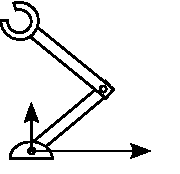
\includegraphics[width=0.27\textwidth]{figs/fwk2dofarm}
  \end{center}
  \caption{A simple 2-DOF arm.\label{fig:fwk2dofarm}}
\end{figure}

Consider a robot arm made out of two links and two joints that is mounted to a table. Let the length of the first link be $l_1$ and the length of the second link be $ l_2$. You could specify the position of the link closer to the table by the angle $ \alpha$ and the angle of the second link relative to the first link using the angle $ \beta$. Suitable conventions and coordinate systems are shown in Figure~\ref{fig:fwk2dofarm}

We can now calculate the position of the joint between the first and the second link using simple trigonometry:

\begin{eqnarray}\label{eq:cosxl1}
x_1 &=&\cos \alpha l_1\\
y_1 &=&\sin \alpha l_1
\end{eqnarray}

Similarly, the position of the end-effector is given by

\begin{eqnarray}
x_2&=&\cos(\alpha+\beta)l_2+x_1\\
y_2&=&\sin(\alpha+\beta)l_2+y_1
\end{eqnarray}
%
or together, the position of the end-effector $(x,y)$ is given by

\begin{eqnarray}\label{eq:cosx}
x&=&\cos(\alpha+\beta)l_2+\cos\alpha l_1\\
y&=&\sin(\alpha+\beta)l_2+\sin\alpha l_1
\end{eqnarray}

The above equations are the kinematic equations of this robot as they relate its control parameters $ \alpha$ and $\beta$ to the position of its end-effector given in the local coordinate system spanned by $ x$ and $ y$ with the origin at the robot's base. Note that both $\alpha$ and $\beta$ shown in the figure are positive: Both links rotate around the z-axis. Using the right-hand rule, the direction of positive angles is defined to be counter-clockwise.

The \emph{configuration space} \index{Configuration space}\index{C-Space (Configuration space)}, i.e., the set of angles each actuator can be set to, of this robot is given by $ \frac{-\pi}{2}<\alpha<\frac{\pi}{2}$ as it is not supposed to run into the table, and $ -\pi < \beta < \pi$. The configuration space is given with respect to the robot's joints and allows us to calculate the \emph{workspace}\index{Workspace} of the robot, i.e., the physical space it can move to, using the forward kinematic equations. This terminology will be identical for mobile robots. An example of configuration and work-space for both a manipulator and a mobile robot is shown in Figure~\ref{fig:holonomy}.

The orientation of the arm's end-effector is given by $\alpha+\beta$. We can now write down  a transformation that includes a rotation around the z-axis
\begin{equation}
\label{eq:2armtrans}
\left(\begin{array}{llll}cos_{\alpha\beta} & -sin_{\alpha\beta} &  0 & \cos_{\alpha\beta}l_2+\cos\alpha l_1\\
                        sin_{\alpha\beta} & cos_{\alpha\beta} & 0 & \sin_{\alpha\beta}l_2+\sin\alpha l_1\\
												0 & 0 & 1 & 0\\
												0 & 0 & 0 & 1\end{array}\right)
\end{equation}
The notation $sin_{\alpha\beta}$ and $cos_{\alpha\beta}$ are short-hand for $sin(\alpha+\beta)$ and $cos(\alpha+\beta)$, respectively.

This transformation now allows us to translate from the robot's base to the robot's end-effector as a function of the actuator positions $\alpha$ and $\beta$. This transformation will be helpful if we want to calculate suitable joint angles in order to reach a certain pose or if we want to convert measurements taken relative to the end-effector back into the base's coordinate system.

\subsection{Forward Kinematics of a Differential Wheels Robot}\label{sec:fwkmobile}
Whereas the pose of a robotic manipulator is uniquely defined by its joint angles---which can be made available using encoders in almost real-time---this is not the case for a mobile robot. Here, the encoder values simply refer to wheel orientation and need to be integrated over time, which will be a huge source of uncertainty as we will later see.
What complicates matters is that for so-called \emph{non-holonomic} systems, it is not sufficient to simply measure the distance that each wheel traveled, but also when each movement was executed.

\begin{figure}[htb!]
	\centering
		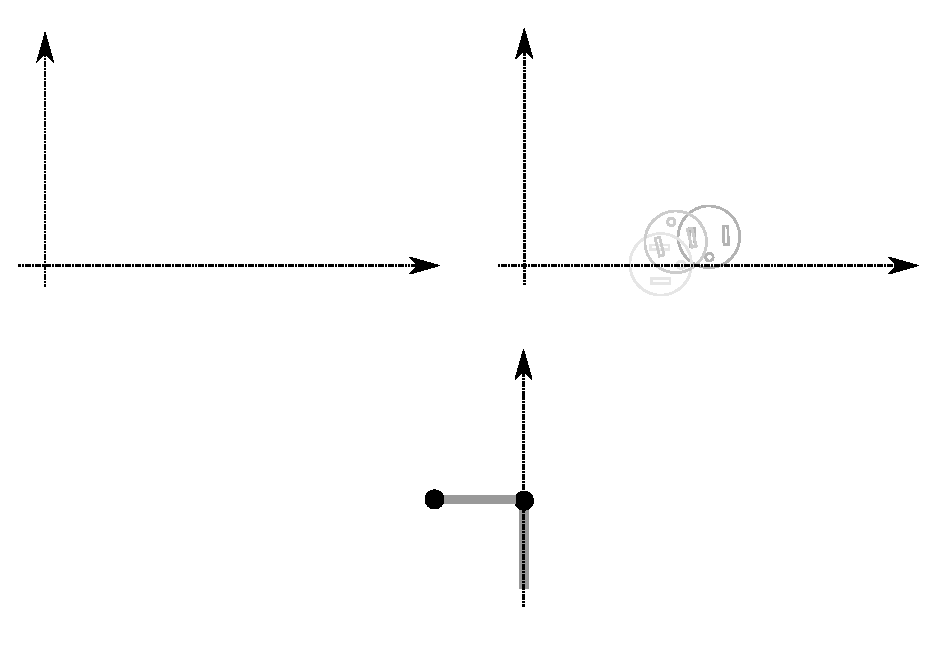
\includegraphics[width=0.95\textwidth]{figs/holonomy.png}
	\caption{Configuration space (left) and workspace (right) for a non-holonomic mobile robot (top) and a holonomic manipulator (bottom). Closed trajectories in configuration space result in closed trajectories in the workspace if the robot's kinematics is holonomic.}
	\label{fig:holonomy}
\end{figure}

A system is non-holonomic\index{Non-holonomic}\index{Holonomic} when closed trajectories in its configuration space (reminder: the configuration space of a two-link robotic arm is spanned by the possible values of each angle) may not have it return to its original state.  A simple arm is holonomic, as each joint position corresponds to a unique position in space. Going through whatever trajectory that comes back to the starting point in configuration space, will put the robot at the exact same position. A train on  a track is holonomic: moving its wheels backwards by the same amount they have been moving forward brings the train to the exact same position in space. A car and a differential-wheel robot are non-holonomic vehicles: performing a straight line and then a right-turn leads to the same amount of wheel rotation than doing a right turn first and then going in a straight line; getting the robot to its initial position requires not only to rewind both wheels by the same amount, but also getting their relative speeds right. The configuration and corresponding workspace trajectories for a non-holonomic and a holonomic robot are shown in Figure~\ref{fig:holonomy}. Here, a robot first moves on a straight line (both wheels turn an equal amount). Then the left wheel remains fixed and only the right wheel turns forward. Then the right wheel remain fixed and the left wheel turns backward. Finally, the right wheel turns backward, arriving at the initial encoder values (zero). Yet, the robot does not return to its origin. Performing a similar trajectory in the configuration space of a two-link manipulator instead, let the robot return to its initial position.

It should be clear by now that for a mobile robot, not only traveled distance per wheel matters, but also the speed of each wheel as a function of time. Instead, this information was not required to uniquely determine the pose of a manipulating arm. Lets introduce the following conventions. We will establish a world coordinate system $\{I\}$, which is known as the inertial frame by convention (Figure~\ref{fig:mobilerobot}). We establish a coordinate system $\{R\}$ on the robot and express the robot's speed $^R\dot{\xi}$ as a vector $ ^R\dot{\xi}=[^R\dot{x}, ^R\dot{y}, ^R\dot{\theta}]^T$. Here $^R\dot{x}$ and $^R\dot{y}$ correspond to the speed along the x and y directions in $\{R\}$, whereas $^R\dot{\theta}$ corresponds to the rotation around the imaginary z-axis, that you can imagine to be sticking out of the ground. We denote speeds with dots over the variable name, as speed is simply the derivative of distance.  Think about the robot's position in $\{R\}$ real quick. It is always zero, as the coordinate system is fixed on the robot. Therefore, velocities are the only interesting quantities in this coordinate system and we need to understand how velocities in $\{R\}$ map to positions in $ \{I\}$, which we denote by $^I\xi=[^Ix, ^Iy, ^I\theta]^T$. These coordinate systems are shown in Figure~\ref{fig:mobilerobot}.

\begin{figure}[htb!]
	\centering
		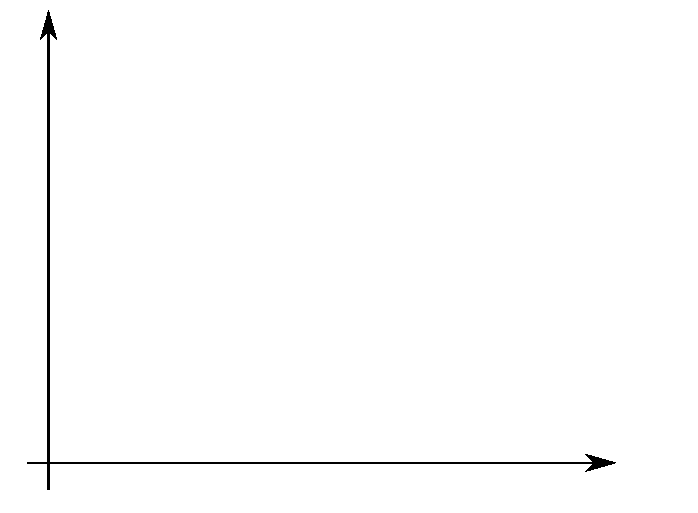
\includegraphics[width=0.85\textwidth]{figs/mobilerobot.png}
	\caption{Mobile robot with local coordinate system \{R\} and world frame \{I\}. The arrows indicate the positive direction of position and orientation vectors.}
	\label{fig:mobilerobot}
\end{figure}



Notice that the positioning of the coordinate frames and their orientation are arbitrary. Here, we chose to place the coordinate system in the center of the robot's axle and align $^Rx$ with its default driving direction.

In order to calculate the robot's position in the inertial frame, we need to first find out, how speed in the robot coordinate frame maps to speed in the inertial frame. This can be done again by employing trigonometry. There is only one complication: a movement into the robot's x-axis might lead to movement along both the x-axis and the y-axis of the world coordinate frame. By looking at the figure above, we can derive the following components to $\dot{x}_I$. First,
\begin{equation}
\dot{x}_{I,x}=cos(\theta) \dot{x}_R.
\end{equation}

There is also a component of motion coming from $ \dot{y}_R$ (ignoring the kinematic constraints for now, see below).  For negative $ \theta$, as in Figure~\ref{fig:mobilerobot}, a move along $y_R$ would let the robot move into positive $ X_I$ direction. The projection from $ \dot{y}_R$ is therefore given by
\begin{equation}
\dot{x_{I,y}}=-sin(\theta)\dot{y_R}.
\end{equation}
We can now write
\begin{equation}
\dot{x_I}=cos(\theta) \dot{x_R} - sin(\theta) \dot{y_R}.
\end{equation}
Similar reasoning leads to
\begin{equation}
\dot{y_I}=sin(\theta) \dot{x_R} + cos(\theta) \dot{y_R}
\end{equation}
and
\begin{equation}
\dot{\theta_I}=\dot{\theta_R}
\end{equation}
which is the case because both robot's and world coordinate system share the same z-axis in this example. We can now conveniently write
\begin{equation}
\dot{\xi_I}=^I_RT(\theta)\dot{\xi_R}
\end{equation}
with
\begin{equation}
^I_RT(\theta)=\left(\begin{array}{ccc}
cos(\theta) & -sin(\theta) & 0 \\
sin(\theta) & cos(\theta) & 0 \\
0 & 0 & 1\end{array}\right)
\end{equation}

We are now left with the problem of how to calculate the speed $ \dot{\xi_R}$ in robot coordinates. For this, we make use of the \emph{kinematic constraints}\index{Kinematic constraints} of the robotic wheels. For a standard wheel, the kinematic constraints are that every rotation of the wheel leads to strictly forward or backward motion and does not allow side-way motion or sliding. We can therefore calculate the forward speed of a wheel $ \dot{x}$ using its rotational speed $ \dot{\phi}$ (assuming the encoder value/angle is expressed as $ \phi$) and radius $ r$ by
\begin{equation}
\dot{x}=\dot{\phi}r.
\end{equation}
This becomes apparent when considering that the circumference of a wheel with radius $r$ is $2\pi r$. The distance a wheel rolls when turned by the angle $ \phi$ (in radians) is therefore $ x=\phi r$, see also Figure~\ref{fig:wheelrotation}, right. Taking the derivative of this expression on both sides leads to the above expression.

\begin{figure}[htb!]
	\centering
		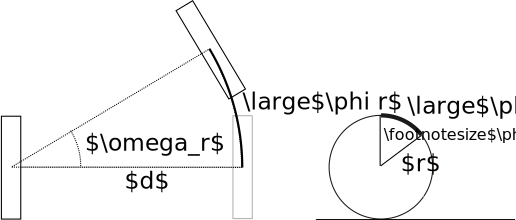
\includegraphics[width=0.9\textwidth]{figs/wheelrotation.png}
	\caption{Left: Differential wheel robot pivoting around its left wheel. Right: A wheel with radius $r$ moves by $\phi r$ when rotated by $\phi$ degrees.}
	\label{fig:wheelrotation}
\end{figure}

How each of the two wheels in our example contributes to the speed of the robot's center---where its coordinate system is anchored---requires the following trick: we calculate the contribution of each individual wheel while assuming all other wheels remaining un-actuated. In this example, the distance traveled by the center point is exactly half of that traveled by each individual wheel, assuming the non-actuated wheel rotating around its ground contact point (Figure~\ref{fig:wheelrotation}). We can therefore write
\begin{equation}
\dot{x_R}=\frac{r\dot{\phi_l}}{2}+\frac{r\dot{\phi_r}}{2}
\end{equation}
given the speeds $ \dot{\phi_l}$ and $ \dot{\phi_r}$ of the left and the right wheel, respectively.

\begin{framed}
Think about how the robot's speed along its y-axis is affected by the wheel-speed given the coordinate system in the drawing above. Think about the kinematic constraints that the standard wheels impose.
\end{framed}

Hard to believe at first, but the speed of the robot along its y-axis is always zero. This is because the constraints of the standard wheel tell us that the robot can never slide.  We are now left with calculating the rotation of the robot around its z-axis. That there is such a thing can be immediately seen when imaging the robot's wheels spinning in opposite directions. We will again consider each wheel independently. Assuming the left wheel to be non-actuated, spinning the right wheel forwards will lead to counter-clockwise rotation. Given an axle diameter (distance between the robot's wheels) $ d$, we can now write
\begin{equation}
\omega_r d = \phi_r r
\end{equation}
with $ \omega_r$ the angle of rotation around the left wheel (Figure~\ref{fig:wheelrotation}, right). Taking the derivative on both sides yields speeds and we can write
\begin{equation}
\dot{\omega_r} = \frac{\dot{\phi_r} r}{d}
\end{equation}
Adding the rotation speeds up (with the one around the right wheel being negative based on the right-hand grip rule), leads to

\begin{equation}
\dot{\theta}=\frac{\dot{\phi_r} r}{d}-\frac{\dot{\phi_l} r}{d}
\end{equation}

Putting it all together, we can write

\begin{equation}\label{eq:diffwheels}
\left(\begin{array}{c} \dot{x_I}\\\dot{y_I}\\\dot{\theta}\end{array}\right)=\left(\begin{array}{ccc}
cos(\theta) & -sin(\theta) & 0 \\
sin(\theta) & cos(\theta) & 0 \\
0 & 0 & 1\end{array}\right)\left(\begin{array}{c}\frac{r\dot{\phi_l}}{2}+\frac{r\dot{\phi_r}}{2}\\0\\\frac{\dot{\phi_r} r}{d}-\frac{\dot{\phi_l} r}{d}\end{array}\right)
\end{equation}

\subsubsection{From Forward Kinematics to Odometry}
Equation~\ref{eq:diffwheels} only provides us with the relationship between the robot's wheel-speed and its speed in the inertial frame. Calculating its actual pose in the inertial frame is known as \emph{odometry}\index{Odometry}. Technically, it requires integrating (\ref{eq:diffwheels}) from 0 to the current time $T$. As this is not possible, but for very special cases, one can approximate the robot's pose by summing up speeds over discrete time intervals, or more precisely
\begin{equation}
\left(\begin{array}{c} {x_I}(T)\\{y_I}(T)\\{\theta}(T)\end{array}\right)=
\int_0^T \left(\begin{array}{c} \dot{x_I}(t)\\\dot{y_I}(t)\\\dot{\theta}(t)\end{array}\right) dt \approx
\sum_{k=0}^{k=T}\left(\begin{array}{c} \Delta{x_I}(k)\\\Delta{y_I}(k)\\\Delta{\theta}(k)\end{array}\right)\Delta t
\end{equation} which can be calculated incrementally as
\begin{equation}\label{eq:odometry}
x_I(k+1)=x_I(k)+\Delta x (k)
\end{equation}
using $\Delta x(k) \approx \dot{x_I}(t)$ and similar expressions for $y_I$ and $\theta$. Note that (\ref{eq:odometry}) is just an approximation. The larger $\Delta t$ becomes, the more inaccurate this approximation becomes as the robot's speed might change during the interval.

\begin{framed}
Don't let the notion of an integral worry you! As robots' computers are fundamentally discrete, integrals usually turn into sums, which are nothing than for-loops.
\end{framed}



\subsection{Forward kinematics of Car-like steering}
Differential wheel drives are very popular in mobile robotics as they are very easy to build, maintain, and control. Although not holonomic, a differential drive can approximate the function of a fully holonomic robot by first driving on the spot to achieve the desired heading and then driving straight. Drawbacks of the differential drive are its reliance on a caster wheel, which performs poorly at high speeds, and difficulties in driving straight lines as this requires both motors to drive at the exact same speed.


These drawbacks are mitigated by car-like mechanisms, which are driven by a single motor and can steer their front wheels. This mechanism is known as ``Ackermann steering'' \index{Ackermann steering}. Ackermann steering should not be confused with ``turntable'' steering \index{Turntable steering} where the front wheels are fixed on an axis with central pivot point. Instead, each wheel has its own pivot point and the system is constrained in such a way that all wheels of the car drive on circles with a common center point, avoiding skid. As the Ackermann mechanism lets all wheels drive on circles with a common center point, its kinematics can be approximated by those of a tricycle with rear-wheel drive, or even simpler by a bicycle. This is shown in Figure~\ref{fig:ackermann}.

\begin{figure}[htb!]
	\centering
		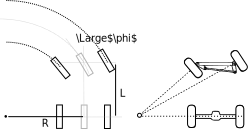
\includegraphics[width=0.9\textwidth]{figs/ackermann.png}
	\caption{Left: Kinematics of car-like steering and the equivalent bicycle model. Right: Mechanism of an Ackermann vehicle.}
	\label{fig:ackermann}
\end{figure}

Let the car have the shape of a box with length $L$ between rear and front axis. Let the center point of the common circle described by all wheels be distance $ R$ from the car's longitudinal center line.  Then, the steering angle $ \phi$ is given by

\begin{equation}\label{eq:ackermann}
\tan \phi = \frac{L}{R}
\end{equation}

The angles of the left and the right wheel, $ \phi_l$ and $ \phi_r$ can be calculated using the fact that all wheels of the car rotate around circles with a common center point. With the distance between the two front wheels $l$, we can write
\begin{eqnarray}
\frac{L}{R-l/2}&=\tan{(\pi/2-\phi_r)}\\
\frac{L}{R+l/2}&=\tan{(\pi/2-\phi_l)}
\end{eqnarray}
This is important, as it allows us to calculate the resulting wheel angles resulting from a specific angle $\phi$ and test whether they are within the constraints of the actual vehicle.

Assuming the wheelspeed to be $\dot{\omega}$ and the wheel radius $r$, we can calculate the speeds in the robot's coordinate frame to
\begin{eqnarray}
\dot{x}_r=\dot{\omega}r\\
\dot{y}_r=0\\
\dot{\theta}_r=\frac{\dot{\omega}r\tan\phi}{L}
\end{eqnarray}
using (\ref{eq:ackermann}) to calculate the circle radius $R$.

\section{Forward Kinematics using the Denavit-Hartenberg scheme}
So far, we have considered the forward kinematics of wheeled mechanisms and simple arms and derived relationships between actuator parameters and velocities using basic trigonometry. In the specific case of multi-link arms, we can also think about the forward kinematics as a chain of homogenous transformations with respect to a coordinate system mounted at the base of a manipulator or a fixed position in the room. Deriving these transformations can be confusing and can be facilitated by following a ``recipe'' such as conceived by Denavit and Hartenberg. The so-called Denavit-Hartenberg (DH) \index{Denavit-Hartenberg parameters}scheme has evolved as quasi-standard and can easily be automatized, i.e., applied to a 3D model of a robotic arm, e.g.

A manipulating arm consists of links that are connected by joints. Joints can be either rotational or prismatic, i.e., change their length and thus providing additional degrees of freedom. Knowing the length of all rigid links, the position of the manipulators end-effector is fully described by its joint angles and joint offset (for prismatic joints).

%In industrial manipulators, the number of joints is usually equal to the degrees of freedom of the manipulator. As most manipulators are holonomic, the forward kinematics allow you---unlike on non-holonomic wheeled platforms---to directly relate absolute positions of joints with absolute positions in Cartesian space. It is also possible to derive equations that relate the speed of the joints to speed in Cartesian space. Like for wheeled platforms, this can be achieved via a Jacobian matrix.  At certain positions, the mapping provided by the Jacobian is not invertible, i.e., some velocities in Cartesian space are unachievable. These points are called singularities.

\screencast{http://youtu.be/rA9tm0gTln8}{denavithartenberg}
In oder to use the DH-convention, we first need to define a coordinate system at each joint. We chose the z-axis to be the axis of rotation for a hinge joint and the axis of translation for a prismatic joint. We can now find the common normal between the z-axes of two subsequent joints, i.e., a line that is orthogonal to each z-axis and intersects both. With the direction of the x-axis at the base arbitrary, subsequent x-axis are chosen such that they lie on the common normal shared between two joints. Whereas the direction of the z-axis is given by the positive direction of rotation (right hand rule), the x-axis points away from the previous joint. This allows defining the y-axis using the right-hand rule. Note that these rules, in particular the requirement that $x$-axes lie along the commom normal, might result in coordinate systems with their origins outside the joint. %Rather, the origin of joint $n$ is at the intersection of

The transformation between two joints is then fully described by the following four parameters:
\begin{enumerate}
\item The length $ r$ of the common normal between the $z$-axes of two joints $i$ and $i-1$ (link length).
\item The angle $ \alpha$ between the z-axes of the two joints with respect to the common normal (link twist), i.e., the angle between the old and the new $z$-axis, measured about the common normal.
\item The distance $d$ between the joint axes (link offset), i.e., the offset along the previous $z$-axis to the common normal.
\item The rotation $ \theta$ around the common axis along which the link offset is measured (joint angle), i.e., the angle from the old $x$-axis to the new $x$-axis, about the previous $z$-axis.
\end{enumerate}

Two of the D-H parameters describe the link between the joints, and the other two describe the link's connection to a neighboring link. Depending on the link/joint type, these numbers are fixed or can be controlled. For example, in a revolute joint $ \theta$ is the varying joint angle, while all other quantities are fixed.  Similarly, for a prismatic joint $ d$ is the joint variable. An example of two revolute joints is shown in Figure~\ref{fig:denavit}.

\begin{figure}
	\centering
		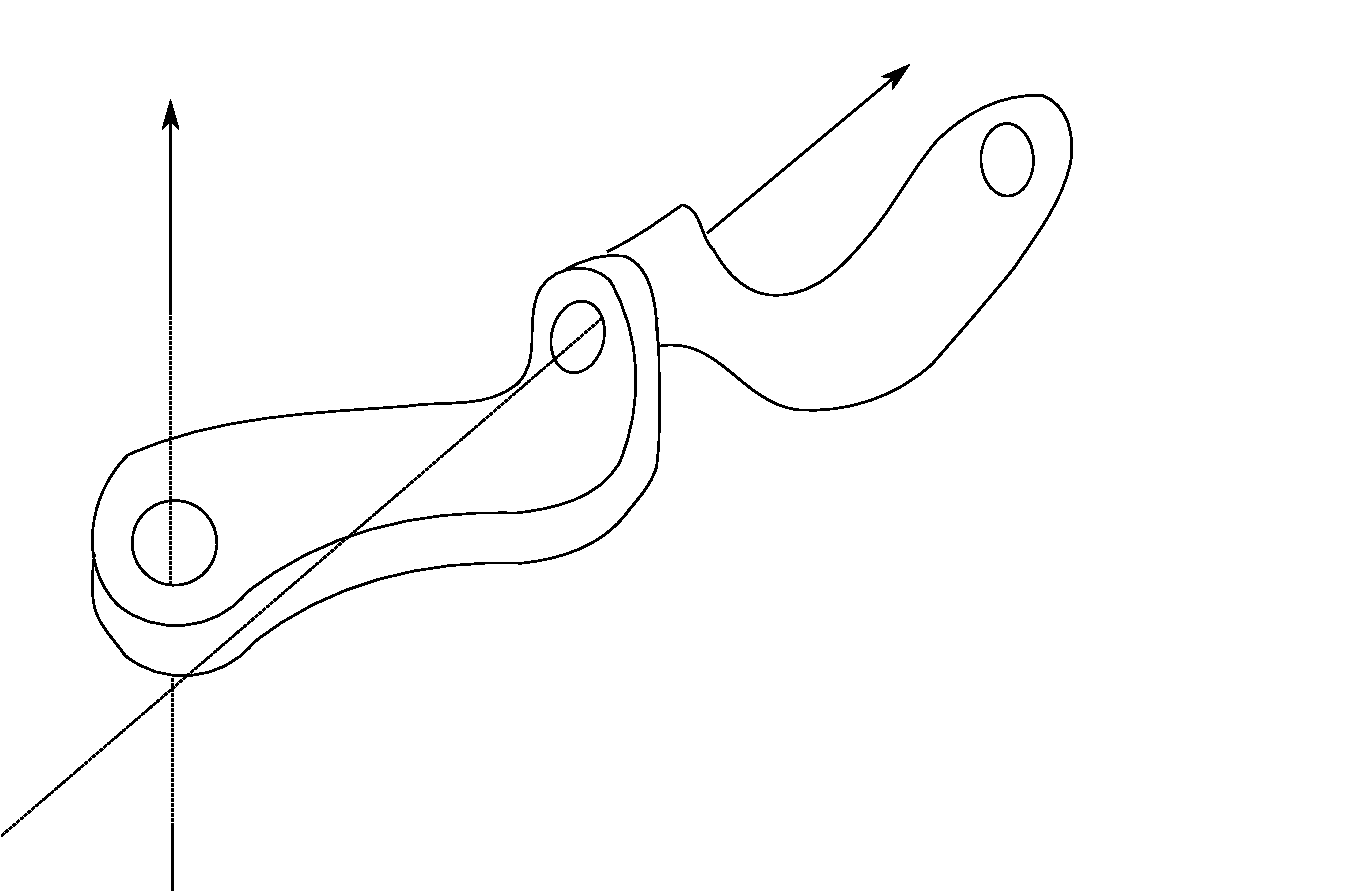
\includegraphics[width=\textwidth]{figs/denavit-hartenberg}
	\caption{Example of selected Denavit-Hartenberg parameters for three revolute joints. The z-axes of joint $i$ and $i+1$ are parallel.
	\label{fig:denavit}}
\end{figure}



The coordinate transform from one link ($ i-1$) to another ($i$) can now be constructed  using the following matrix:
\begin{eqnarray}{ll}
\nonumber
_{n-1}^nT=&
\left(
\begin{array}{ccc|c}
\cos \theta_n & -\sin \theta_n \cos\alpha_n & \sin\theta_n \sin\alpha_n & r_n \cos\theta_n\\
\sin \theta_n & \cos\theta_n \cos\alpha_n & -\cos\theta_n\sin\alpha_n & r_n \sin\theta_n\\
0 & \sin\alpha_n & \cos\alpha_n & d_n\\
\hline
0 & 0 & 0 & 1
\end{array}
\right)\\
&=
\left(
\begin{array}{c|c}
R & t\\
\hline
0 \quad 0 \quad 0 & 1
\end{array}
\right)
\end{eqnarray}
with the rotation matrix $R$ and the translation vector $t$. This matrix can be constructed by a series of rotations and translations, one for each DH parameter:
\begin{equation}
_{n-1}^nT=T_z'(d_n)\dot R_z'(\theta_n) \dot T_x(r_n) \dot R_x(\alpha_n)
\end{equation}
with
\begin{equation}
T_z'(d_n)=
\left(
\begin{array}{ccc|c}
1 & 0 & 0 & 0\\
0 & 1 & 0 & 0\\
0 & 0 & 1 & d_n\\
\hline
0 & 0 & 0 & 1
\end{array}
\right)
\enskip
R_z'(\theta_n)=\left(
\begin{array}{ccc|c}
\cos\theta_n & -\sin\theta_n & 0 & 0\\
\sin\theta_n & \cos\theta_n & 0 & 0\\
0 & 0 & 1 & 0\\
\hline
0 & 0 & 0 & 1
\end{array}
\right)
\end{equation}
and
\begin{equation}
T_x(r_n)=
\left(
\begin{array}{ccc|c}
1 & 0 & 0 & r_n\\
0 & 1 & 0 & 0\\
0 & 0 & 1 & 0\\
\hline
0 & 0 & 0 & 1
\end{array}
\right)
\enskip
R_x(\alpha_n)=\left(
\begin{array}{ccc|c}
1 & 0 & 0 & 0\\
0 & \cos\alpha_n & -\sin\alpha_n & 0\\
0 & \sin\alpha_n & \cos\alpha_n & 0\\
\hline
0 & 0 & 0 & 1
\end{array}
\right)
\end{equation}
These are a translation of $d_n$ along the previous z-axis ($T_z'(d_n)$), a rotation of $\theta_n$ about the previous z-axis ($R_z'(\theta_n)$), a translation of $r_n$ along the new $x$-axis ($T_x(r_n)$)and a rotation of $\alpha_n$ around the new $x$-axis ($R_x(\alpha_n)$).

Like for any homogeneous transfrom, the inverse $_{n-1}^nT^{-1}n$ is given by
\begin{equation}
^{n-1}_nT=\left(
\begin{array}{c|c}
R^{-1} & -R^{-1}T\\
\hline
0 \quad 0 \quad 0 \quad 1
\end{array}
\right)
\end{equation}
with the inverse of $R$ simply being its transpose.
